\section{Jazyk C}
C je programovací jazyk, který počátkem 70. let 20. století vyvinuli Ken Thompson a Dennis Ritchie pro potřeby operačního systému Unix. Jde o vyšší programovací jazyk, který přesto umožňuje zapisovat programové konstrukce tak, jak je počítač skutečně zpracovává, takže výsledný kód může být velmi efektivní, a proto v minulosti nahradil nízkoúrovňový jazyk symbolických adres. Jazyk C je kompilovaný, imperativní, procedurální, strukturovaný, podporuje rekurzi, má statickou typovou kontrolu. Je využíván pro programování operačního systému a aplikačního software od superpočítačů k PLC a vestavěných systémů.

\subsection{Vývojové prostředí Dev C++}
Dev-C++ je svobodné vývojové prostředí vyvinuté společností Bloodshed software pro C a C++. Je určeno pro operační systém MS Windows a jako překladač používá MinGW, klon GCC. Dev-C++ je také možné používat spolu s prostředím Cygwin nebo jinými překladači založenými na GCC.

\subsection{Preprocesor}
Preprocesor je počítačový program, který zpracovává vstupní data tak, aby výstup mohl dále zpracovávat jiný program. Preprocesor je často používán pro předzpracování zdrojového kódu před vlastní kompilací. Druh a míra předzpracování závisí zejména na schopnostech preprocesoru. Většina preprocesorů je relativně jednoduchá, zvládá nahrazování textu a jednoduchá makra. Existují též sofistikované preprocesory, případně plně rozvinuté programovací jazyky.

\subsection{Compiler}
Překladač (kompilátor) je v nejčastějším smyslu slova softwarový nástroj používaný programátory pro vývoj softwaru. Kompilátor slouží pro překlad algoritmů zapsaných ve vyšším programovacím jazyce do jazyka nižšího, nejčastěji strojového, či spíše do strojového kódu. Z širšího obecného hlediska je kompilátor stroj, respektive program, provádějící překlad z nějakého vstupního jazyka do jazyka výstupního.

\subsection{Assembler}
Assembler je počítačový program, který slouží k překladu programu napsaného v jazyce symbolických adres (JSA) do strojového kódu, tedy posloupnosti strojových instrukcí vykonávaných procesorem počítače. Jako „assembler“ se přeneseně označuje i samotný jazyk symbolických adres (anglicky assembly language).

\subsection{Linker}
Linker je počítačový program, který jeden nebo více objektových souborů vygenerovaných překladačem spojí do jediného spustitelného souboru (tzv. linkování). Výsledný soubor může být přímo spustitelný jádrem operačního systému nebo knihovnou, která je později využívána jiným programem. Statická knihovna je připojována k jinému programu, dynamická knihovna je s programem spojována při jeho zavádění do paměti (zavaděč vyvolá dynamický linker).

\begin{figure}[htbp]
\centering
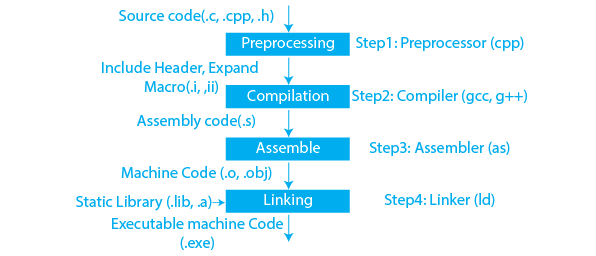
\includegraphics[scale=0.5]{sections/1_jazyk_c/images/1679577255149-1-02 (15).png}
\end{figure}
\subsection{Datové typy}
\paragraph{Definice}
Definice proměnné znamená, že je v paměti alokován prostor pro tuto proměnnou. Při definici proměnné je také určeno její jméno a datový typ. Definice může, ale nemusí zahrnovat inicializaci.
int a - Definice.
int a = 10 - Definice s deklarací.
\paragraph{Inicializace}
Inicializace proměnné znamená, že jí přiřadíte počáteční hodnotu při jejím vzniku. Inicializace může proběhnout buď současně s definicí, nebo později. int d. d = 10.
\paragraph{Přetypování}
Přetypování (anglicky "type casting") v jazyce C umožňuje převést hodnotu z jednoho datového typu na jiný. Toto je užitečné v situacích, kdy je potřeba provést operace mezi různými datovými typy nebo uložit hodnotu jednoho typu do proměnné jiného typu
\paragraph{Celočíselné datové typy}
\begin{center}
\begin{tabular}{ |c|c|c| } 
 \hline
 Datový typ & Rozsah & Velikost \\ 
 char & -128 až 127 & 8 bitů \\ 
 short & -32 768 až 32 767 & 16 bitů\\ 
 int & -32 768 až 32 767 nebo -2 147 483 648 až 2 147 483 647 & 16 nebo 32 bitů\\ 
 long int & -2 147 483 648 až 2 147 483 647 & 32 bitů\\ 
 long long int & -9 223 372 036 854 775 808 až 9 223 372 036 854 775 807 & 64 bitů\\ 
 \hline
\end{tabular}
\end{center}
\paragraph{Desetinná čísla}
\begin{center}
\begin{tabular}{ |c|c|c|c| } 
 \hline
  Datový typ & Rozsah & Velikost & Přesnost \\ 
  float & 1.2E-38 až 3.4E+38 & 32 bitů & 6 číslic\\ 
  double & 2.3E-308 až 1.7E+308 & 64 bitů & 15 číslic\\ 
  long double & 3.4E-4932 až 1.1E+4932 & 80 bitů & 19 číslic\\ 
 \hline
\end{tabular}
\end{center}

\paragraph{Unsigned}
Většinu datových typů můžeme ještě předsadit klíčovým slovem
unsigned, např. vytvoříme proměnnou typu
unsigned int a podobně. Sign označuje znaménko čísla a unsigned znamená,
že číslo znaménko nemůže obsahovat. Výsledkem je, že je taková
proměnná vždy nezáporná a vejde se do ni proto i 2x větší číslo,
jelikož není využita záporná část. Nefunguje pro desetinná čísla.
\paragraph{void}
Sám o sobě existovat nemůže. Nejčastěji se používá například jako návratová hodnota funkcí (nevrací nic) nebo jako void* ptr.
\subsection{Standardní vstup a výstup}
Standardní vstup, standardní výstup a standardní proudy obecně je v informatice koncept, který poskytuje každému programu sadu okamžitě použitelných rozhraní pro výstup a vstup dat, obvykle v textovém tvaru. Vychází z pozorování, že většina programů určených pro prostředí příkazového řádku potřebuje někam vypisovat své výsledky, a z myšlenky, že výstup jednoho programu je často vhodné zpracovat jiným programem.

\paragraph{Standardní vstup}
Standardní vstup je standardizované rozhraní, kterým data vstupují do programu. Data na standardním vstupu program principielně může ignorovat, např. tehdy, když je spuštěn s neplatnou kombinací parametrů; programy, které se standardním vstupem nepracují, kupř. ty, jejichž agendou je kopírování, přejmenování, přesunování nebo mazání souborů, datům na něm pozornost nevěnují v principu nikdy.

O přesun dat ze standardního vstupu do paměťového prostoru programu tento žádá použitím operace (systémového volání) read nad souborovým deskriptorem 0. Pojmenování souborového deskriptoru standardního vstupu ve standardní knihovně jazyka C pro práci se vstupem a výstupem (stdio.h) je stdin a v obdobné knihovně jazyka C++ (iostream) je pro tento účel vyhrazen identifikátor std::cin.
\paragraph{Standardní výstup}
Standardní výstup je standardizované rozhraní pro předávání výstupních dat. Žádný program není povinen data na standardní výstup zapisovat; to bez ohledu na vstupní data a parametry, s nimiž byl spuštěn. Existují programy, jež pracují se standardním vstupem a nepoužívají standardní výstup, i programy, které ignorují standardní vstup a jejichž plody odcházejí standardním výstupem; příkladem prvního případu může být klient systému řízení báze dat, který příkazy přijaté ze standardního vstupu vykoná nad databází, za příklad druhého extrému lze pokládat program pro výpis obsahu adresáře.

O to, aby data skrze standardní výstup převzal operační systém, jej program žádá uplatněním operace (systémového volání) write nad souborovým deskriptorem 1. Identifikátor standardního výstupu ve stdio.h je stdout, v iostream tomuto proudu odpovídá označení std::cout.

\subsection{Řídící struktury}
Řídící konstrukce jsou syntaktické prvky umožňující řízení běhu programu, tj. větvení na základě ne/splnění podmínek, opakování úseku kódu (Cykly) a skoky v kódu.
\subsubsection{Větvení}
If, else, switch.
\begin{lstlisting}[style=mystyle]
#include <iostream>
using namespace std;

int main() {
    int a = 10;
    int b = 20;

    // if condition: checks if a is less than b
    if (a < b) {
        cout << "if condition: a is less than b" << endl;
    } 
    // else condition: executed if a is not less than b
    else {
        cout << "else condition: a is not less than b" << endl;
    }

    int c = 2;

    // switch condition: checking the value of c
    switch (c) {
        case 1:
            cout << "switch case 1: c is 1" << endl;
            break;
        case 2:
            cout << "switch case 2: c is 2" << endl;
            break;
        case 3:
            cout << "switch case 3: c is 3" << endl;
            break;
        default:
            cout << "switch default: c is not 1, 2, or 3" << endl;
            break;
    }

    return 0;
}
\end{lstlisting}
\subsubsection{Cykly}
While, do-while, for.

\begin{lstlisting}[style=mystyle]
#include <iostream>
using namespace std;

int main() {
    // for loop: iterates from 0 to 4
    for (int i = 0; i < 5; i++) {
        cout << "for loop, i: " << i << endl;
    }

    int j = 0;
    // while loop: continues while j is less than 5
    while (j < 5) {
        cout << "while loop, j: " << j << endl;
        j++;
    }

    int k = 0;
    // do-while loop: always executes at least once
    do {
        cout << "do-while loop, k: " << k << endl;
        k++;
    } while (k < 5);

    return 0;
}
\end{lstlisting}

\subsection{Práce s polem}
V jazyce C je pole datová struktura, která umožňuje ukládat a manipulovat s více prvky stejného datového typu. Pole v C je také známé jako kontinuální oblast paměti, kde jsou prvky uspořádány za sebou bez mezery.
\begin{lstlisting}[style=mystyle]
#include <stdio.h>

int main() {
    // Declare an array of integers with size 5
    int array[5];

    // Initialize the elements of the array
    array[0] = 10;
    array[1] = 20;
    array[2] = 30;
    array[3] = 40;
    array[4] = 50;

    // Print the elements of the array
    for (int i = 0; i < 5; i++) {
        printf("array[%d] = %d\n", i, array[i]);
    }

    return 0;
}
\end{lstlisting}

\subsection{Algoritmy třídění pole}
\paragraph{Bubble sort}
Bublinkové řazení je jednoduchý třídící algoritmus, který opakovaně prochází seznamem, porovnává sousední prvky a vyměňuje je, pokud jsou ve špatném pořadí. Tento proces se opakuje, dokud není seznam seřazen. Algoritmus získal své jméno podle toho, že největší prvky "bublají" na konec seznamu. Bublinkové řazení je jednoduché na implementaci, ale je pomalé pro velké množiny dat s časovou složitostí $O({n^2})$.
\begin{lstlisting}[style=mystyle]
// Function to perform bubble sort
void bubbleSort(int arr[], int n) {
    int i, j, temp;
    // Loop through the array multiple times
    for (i = 0; i < n-1; i++) {
        // Last i elements are already in place
        for (j = 0; j < n-i-1; j++) {
            // Swap if the element found is greater than the next element
            if (arr[j] > arr[j+1]) {
                temp = arr[j];
                arr[j] = arr[j+1];
                arr[j+1] = temp;
            }
        }
    }
}
\end{lstlisting}

\paragraph{Insertion sort}
Vkládací řazení je jednoduchý třídící algoritmus, který buduje konečný seřazený seznam jeden prvek po druhém. Každý nový prvek se vkládá do správné pozice v již seřazené části seznamu. Algoritmus opakovaně posunuje větší prvky směrem doprava, aby udělal místo pro aktuální prvek. Vkládací řazení je efektivní pro malé množiny dat a má časovou složitost $O(n^2)$ v nejhorším případě, ale je relativně rychlé pro téměř seřazené seznamy.
\begin{lstlisting}[style=mystyle]
// Function to perform insertion sort
void insertionSort(int arr[], int n) {
    int i, key, j;
    for (i = 1; i < n; i++) {
        key = arr[i];
        j = i - 1;

        // Move elements of arr[0..i-1], that are greater than key, to one position ahead of their current position
        while (j >= 0 && arr[j] > key) {
            arr[j + 1] = arr[j];
            j = j - 1;
        }
        arr[j + 1] = key;
    }
}
\end{lstlisting}
\paragraph{Selection sort}
Výběrové řazení je jednoduchý třídící algoritmus, který pracuje tak, že opakovaně hledá nejmenší (nebo největší) prvek z nesetříděné části seznamu a umísťuje jej na správnou pozici ve setříděné části seznamu. Proces se opakuje, dokud nejsou všechny prvky setříděny. Výběrové řazení je snadné na pochopení a implementaci, ale je neefektivní pro velké množiny dat s časovou složitostí $O(n^2)$, protože vždy prochází celým seznamem.
\begin{lstlisting}[style=mystyle]
// Function to perform selection sort
void selectionSort(int arr[], int n) {
    int i, j, min_idx, temp;
    // One by one move the boundary of the unsorted subarray
    for (i = 0; i < n-1; i++) {
        // Find the minimum element in the unsorted array
        min_idx = i;
        for (j = i+1; j < n; j++) {
            if (arr[j] < arr[min_idx]) {
                min_idx = j;
            }
        }
        // Swap the found minimum element with the first element
        temp = arr[min_idx];
        arr[min_idx] = arr[i];
        arr[i] = temp;
    }
}
\end{lstlisting}
\subsection{Funkce}
Funkce v jazyce C je blok kódu, který provádí určitou úlohu a může být volán z jiných částí programu. Funkce může přijímat vstupy (parametry) a vracet výstup (návratovou hodnotu). Použití funkcí umožňuje rozdělit program na menší, spravovatelné části a zvyšuje znovupoužitelnost kódu.
\begin{lstlisting}[style=mystyle]
    int sum(int a, int b); //Deklarace

    int sum(int a, int b) { //Definice
        return a + b;
    }
\end{lstlisting}
Deklarace funkce na začátku umožňuje její použití před její definicí.

\subsection{Struktury a ukazatele}
V jazyce C jsou struktury (structures) a ukazatele (pointers) základními stavebními kameny pro vytváření komplexních datových struktur. Níže je uvedeno vysvětlení obou konceptů a jejich příklad v kódu.
\paragraph{Struktury}
Struktura je uživatelsky definovaný typ dat, který umožňuje seskupení různých typů dat do jednoho celku. Struktury se používají k reprezentaci složitějších datových objektů, které obsahují více různých atributů.
\begin{lstlisting}[style=mystyle]
    struct Person {
        char name[50];
        int age;
        float height;
    };
\end{lstlisting}

\paragraph{Ukazatele}
Ukazatel je proměnná, která obsahuje adresu jiné proměnné. Ukazatele jsou mocným nástrojem pro manipulaci s pamětí, dynamické alokace paměti, a pro práci s datovými strukturami, jako jsou pole a struktury.
\begin{lstlisting}[style=mystyle]
    int a = 10;
    int b = 20;
    int *p = &a;  // Pointer 'p' points to the address of variable 'a'

    // Print the value and address of variable 'a' using pointer
    printf("Value of a: %d\n", a);  // Prints the value of 'a'
    printf("Address of a: %p\n", (void*)&a);  // Prints the address of 'a'
    printf("Value pointed to by p: %d\n", *p);  // Prints the value pointed to by 'p'
    printf("Address stored in p: %p\n", (void*)p);  // Prints the address stored in 'p'
\end{lstlisting}
\subsection{Práce se soubory}
Práce se soubory v jazyce C je důležitá činnost, která umožňuje programům číst data ze souborů, zapisovat do nich nebo je upravovat
\begin{lstlisting}[style=mystyle]
    FILE *fp;  // File pointer

    // Open file for writing ("w" mode)
    fp = fopen("data.txt", "w");

    // Write to file
    fprintf(fp, "Hello, world!\n");

    // Close file
    fclose(fp);

    // Open file for reading ("r" mode)
    fp = fopen("data.txt", "r");

    // Read and print file contents
    char buffer[100];
    printf("File contents:\n");
    while (fgets(buffer, sizeof(buffer), fp) != NULL) {
        printf("%s", buffer);
    }

\end{lstlisting}

\subsection{Knihovny}

\paragraph{stdio.h - Standard Input/Output Library}
Obsahuje funkce pro základní vstup a výstup, například printf, scanf, fopen, fclose pro práci se soubory.

\paragraph{stdlib.h - Standard Library}
Poskytuje funkce pro správu paměti (malloc, free), manipulaci se řetězci (atoi, itoa), a další.

\paragraph{string.h - String Library}
Obsahuje funkce pro manipulaci s řetězci, jako jsou strcpy, strcat, strlen, strcmp.

\paragraph{math.h - Mathematics Library}
Obsahuje matematické funkce, jako jsou sqrt, sin, cos, pow, abs.

\paragraph{Vytváření vlastních knihoven}
Vytváření vlastních knihoven v jazyce C je užitečný způsob, jak organizovat a znovupoužívat části kódu ve vašich projektech. Tento proces obvykle zahrnuje vytvoření hlavičkového souboru (.h) a zdrojového souboru (.c), které obsahují funkce a datové typy určené k opakovanému použití.